\documentclass[instructornotes]{ximera}

%\usepackage{microtype}
%\usepackage{tikz}
\usepackage{tkz-euclide}
%\usetkzobj{all}
\tikzstyle geometryDiagrams=[rounded corners=.5pt,ultra thick,color=blue!50!black]

\usepackage{tikz-cd}

\colorlet{penColor}{blue!50!black} % Color of a curve in a plot

%% \hypersetup{
%%     colorlinks = false,
%%     }


\tikzset{%% partial ellipse
    partial ellipse/.style args={#1:#2:#3}{
        insert path={+ (#1:#3) arc (#1:#2:#3)}
    }
}

\graphicspath{
{./}
{sphericalLunesAndTriangles/}
{hyperbolicLunesAndTriangles/}
{centralProjection/}
{stereographicProjection/}
{linesAnglesAndAreasInCentralProjection/}
{linesAnglesAndAreasInStereographicProjection/}
{stereographicProjection/}
{centralProjectionInHG/}
{stereographicProjectionInHG/}
{linesInSphericalGeometry/}
{linesInHyperbolicGeometry/}
{theArtOfEscher/}
}


\newcommand{\transpose}{\intercal}
\newcommand{\eval}[1]{\bigg[ #1 \bigg]}

\renewcommand{\epsilon}{\varepsilon}
\renewcommand{\l}{\ell}
\renewcommand{\d}{\,d}

\DeclareMathOperator{\arccosh}{arccosh}
\DeclareMathOperator{\arctanh}{arctanh}
\renewcommand{\tilde}{\widetilde}
\newcommand{\R}{\mathbb R}
\newcommand{\dd}[2][]{\frac{d #1}{d #2}}
\newcommand{\pp}[2][]{\frac{\partial #1}{\partial #2}}
\newcommand{\dfn}{\textbf}

\renewcommand{\bar}{\overline}
\renewcommand{\hat}{\widehat}


\ifxake
\NewEnviron{freeResponse}{}
\fi

%% \prerequisites{rigidMotions,geometry}
%% \outcome{Knowledge of neutral geometry.}

\title{Euclid's postulates for plane geometry} % the title of the activity
\begin{document}
\begin{abstract}
We begin with Euclid's first four assumptions and explore neutral
geometries.
\end{abstract}
\maketitle

%% test for svg-viewer
%%
%% \begin{center}
%%   \begin{tikzpicture}
%%     \draw[thick] (0,0) -- (1,1);
%%   \end{tikzpicture}
%% \end{center}



\section{Neutral geometry}

\begin{listOutcomes}
\item State the axioms of neutral geoemtry.
\item State the SAS congruence axiom.
\item Apply SAS.
\item Prove that the sum of the interior angles of a triangle in
  neutral geoemtry is always less than or equal to $180^\circ$.
\end{listOutcomes}

\begin{listOutcomes}
\item State the axioms of neutral geoemtry.
\item State the side-angle-side congruence axiom.
\item Apply side-angle-side.
\item Prove that the sum of the interior angles of a triangle in
  neutral geomtry is always less than or equal to $180^\circ$.
\end{listOutcomes}


%% We first turn our attention to plane (or `flat') two-dimensional
%% geometry.

In Western civilization, the primary source of our understanding of
plane geometry comes from Euclid's \textit{Elements}. The treatise is
of transcendent importance well beyond geometry itself. It is among
the first examples of formal logical deductive reasoning. Certain
fundamentals, that are called \textit{axioms}, are postulated or
`given,' providing the platform on which a `geometry' is built. This
creates a mathematical entity modeling a physical `reality.' Its
properties are arrived at by applying the laws of logic to the given
fundamentals. Euclid gives five axioms for plane geometry, the first
four of which seem to be `obvious' reflections of physical reality. In
paraphrased form, they are:

\begin{axiom}[E1]
Through any point $P$ and any other point $Q$, there lies a unique
line.
\end{axiom}

\begin{axiom}[E2] 
Given any two segments $\bar{AB}$ and $\bar{CD}$, there is a
segment $\bar{AE}$ such that $B$ lies on $\bar{AE}$ and
$\left\vert CD\right\vert =\left\vert BE\right\vert$.

Note: We will use both $\left\vert AB\right\vert$ and $d(A,B)$ to
denote the distance between two points $A$ and $B$.
\end{axiom}

\begin{axiom}[E3]
Given a point $P$ and any positive real number $r$, there exists a
(unique) circle of radius $r$ and center $P$. 

Said another way, if you move away from point $P$ along a line in any
direction, you will encounter a unique point at distance $r$ from $P$.
\end{axiom}

\begin{axiom}[E4]
All right angles are congruent.

Note: A right angle is defined as follows. Let $C$ be the midpoint on
the segment $\bar{AB}$. Let $E$ be any point not equal to
$C$. The angle $\angle ACE$ is called a right angle if $\angle ACE$ is
congruent to $\angle ECB$. [MJG,17-18]
\end{axiom}

\begin{definition}
If we are only given axioms E1--E4, we will call our
geometry \textbf{neutral geometry} (\textbf{NG}).
\end{definition}

\begin{definition}
In \textbf{neutral geometry}, two distinct lines are called \textbf{parallel} if and
only if they don't intersect.
\end{definition}



\begin{definition} 
We will call the set of points on a line which lie on one side of a
given point a \textbf{ray}.  We call the given point the
\textbf{origin} of the ray.
\end{definition}

\begin{remark}
 Spheres do not have neutral geometry. There are infinitely many lines between the north pole and south pole; you can see some of them in this image from Wikipedia:
 
\begin{figure}[h]
 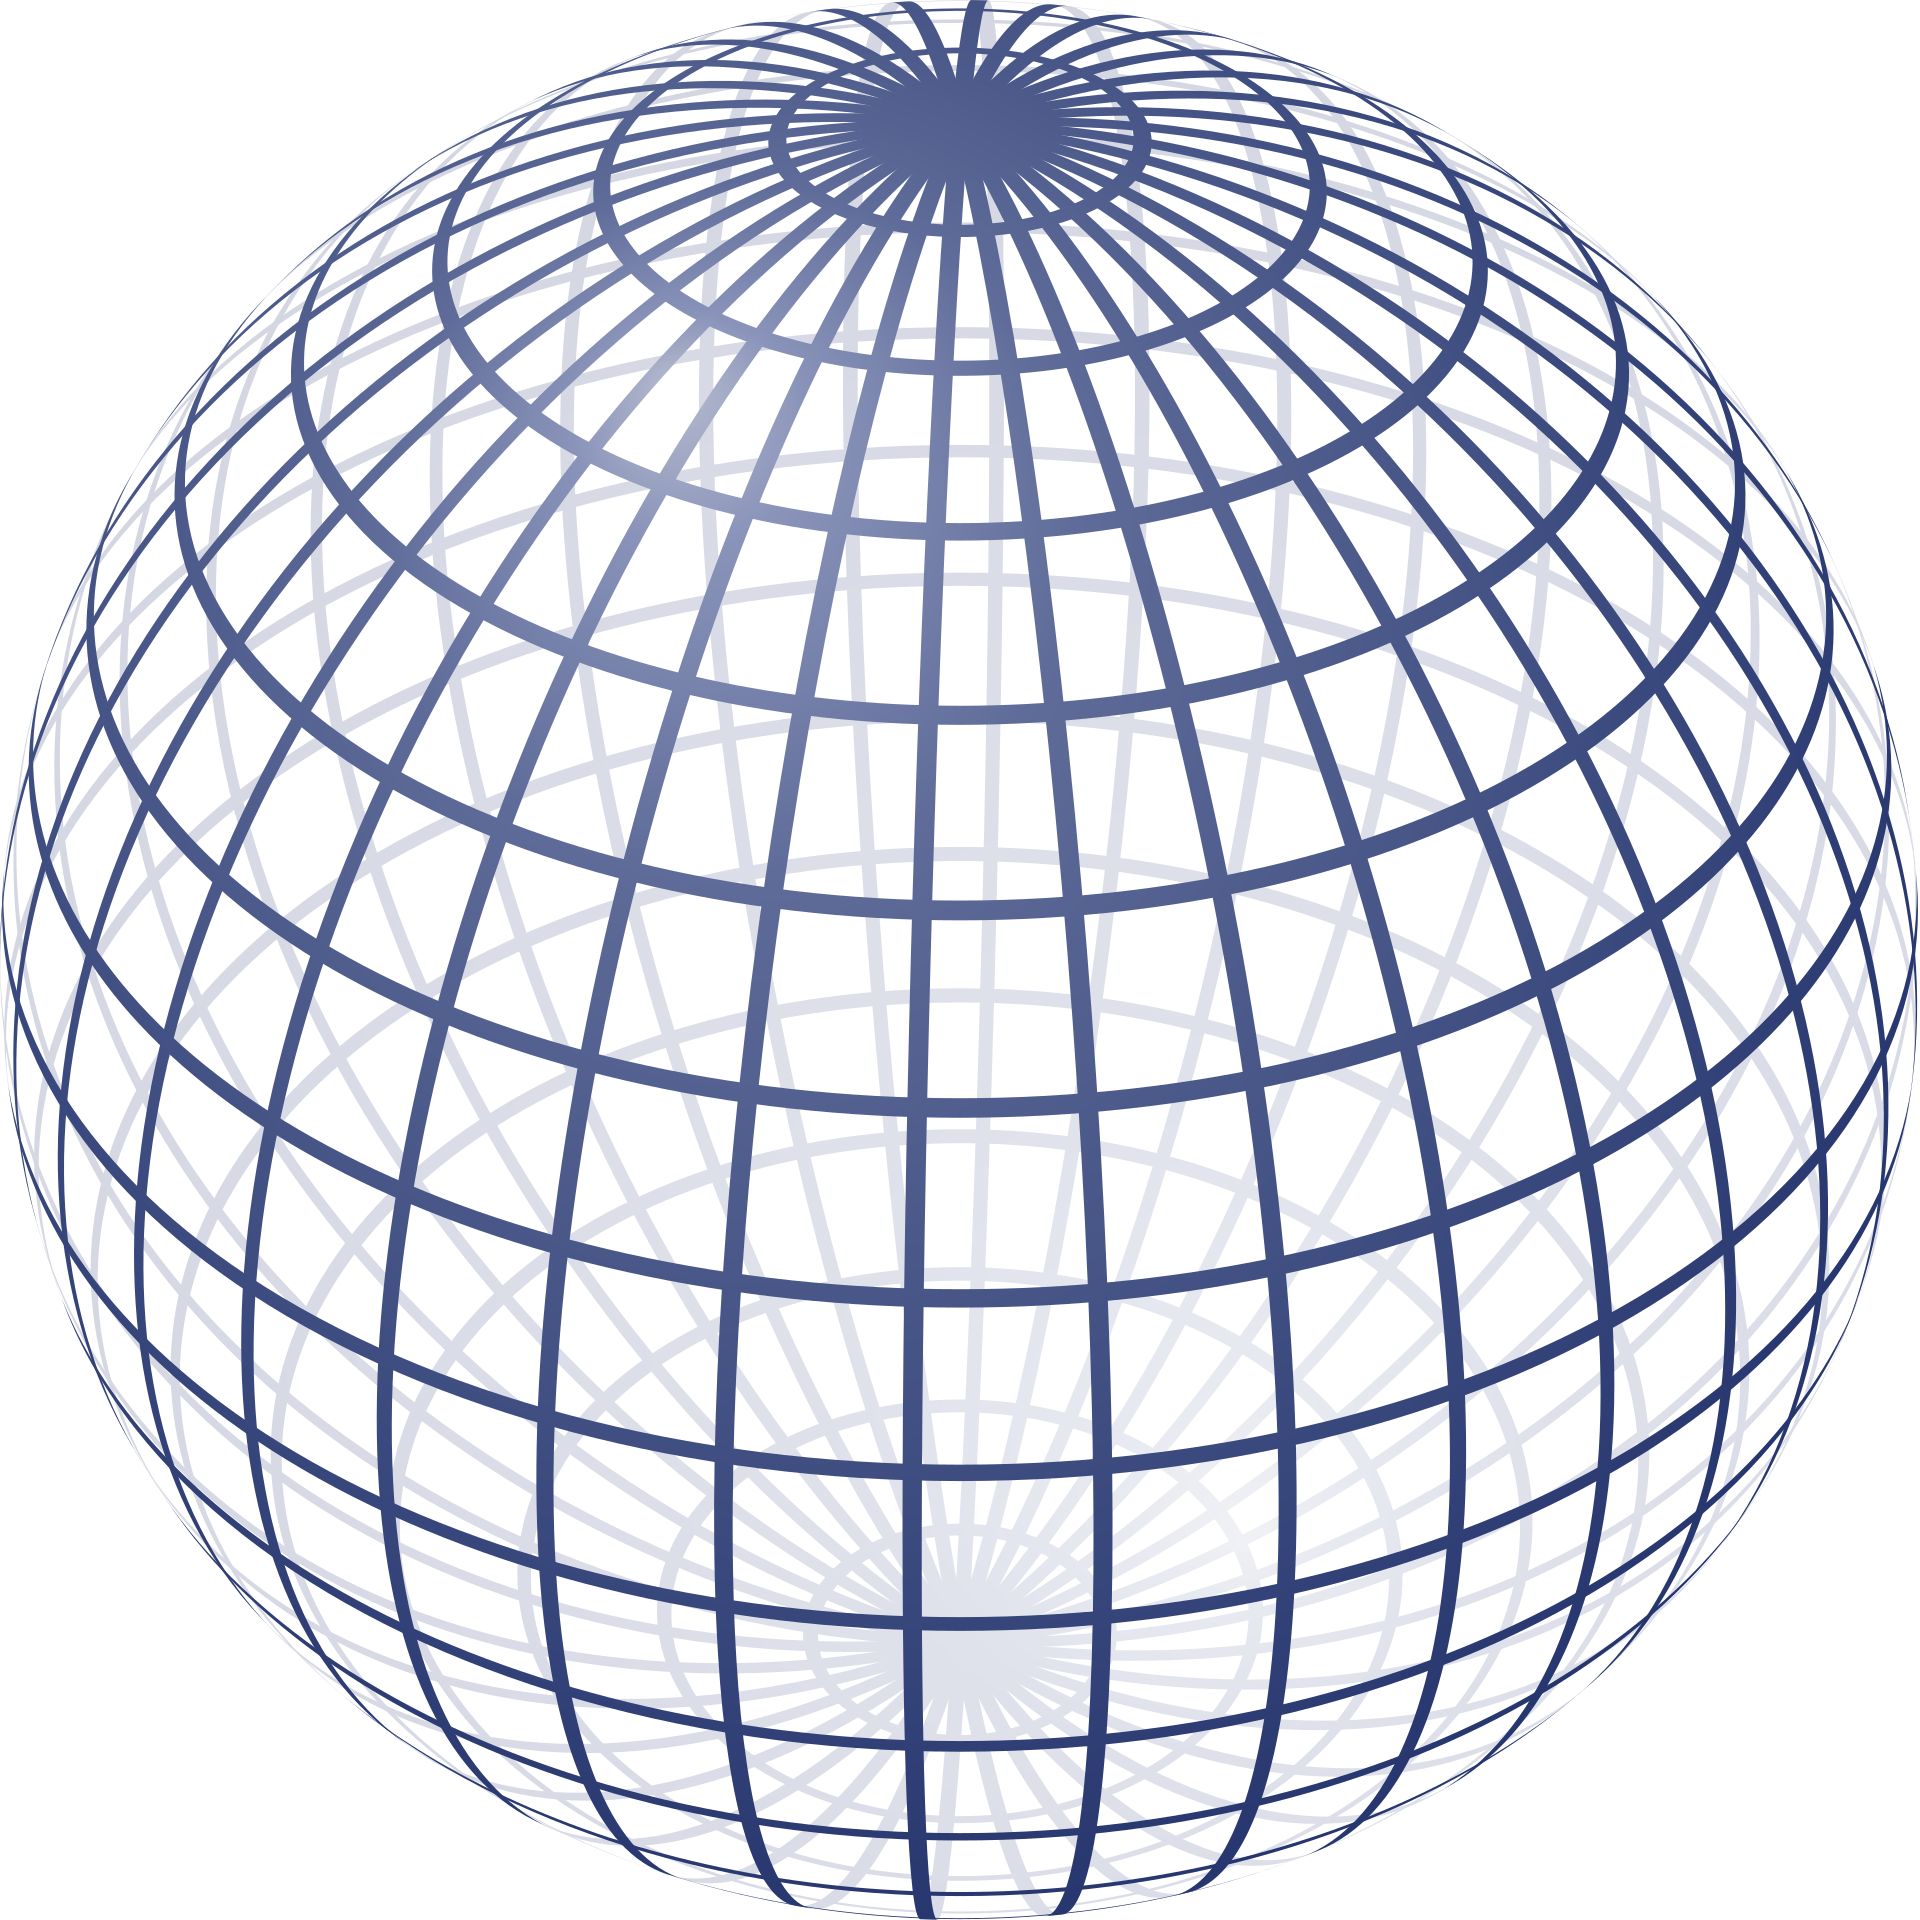
\includegraphics[width=.5\textwidth]{euclidsPostulatesForPlaneGeometry/Sphere.png}
\caption{Image of a wireframe sphere from \url{https://en.wikipedia.org/wiki/Sphere}. By Geek3 - Own work, CC BY 3.0, %\url{https://commons.wikimedia.org/w/index.php?curid=8089933}
}
\end{figure}
\end{remark}

\begin{definition}
We call two rays in the plane \textbf{parallel} if they lie on
parallel lines and they both lie on the same side of the transversal
line passing through their origins.
\end{definition}

\begin{definition} An \textbf{angle} in the plane is the union of two ordered
rays with common origin and choice of one of the two connected regions
into which the union of the rays divides the plane. We often denote
angles by $\angle BAC$ where $A$ is the common origin and $B$ a point
along one of the rays, called the initial ray, and $C$ is a point
along the other ray, called the final ray.
\end{definition}


The choice of the region is either clear from the context or
explicitly given.

\begin{problem}
Given an angle $\angle BAC$ show by drawings the two regions into
which it divides the plane. Show how the (signed) measure of the angle
depends on:
\begin{enumerate}
\item Which region you pick as the interior/exterior. 
\item Which ray is the initial ray and which is the final ray of the
  angle.
\end{enumerate}
\begin{freeResponse}
We present a summary in the table below:
\begin{center}
\begin{tabular}{|c|c|}\hline
%\begin{image}
\begin{tikzpicture}[geometryDiagrams]
\coordinate (A) at (0,0);
\coordinate (B) at (2,2);
\coordinate (C) at (2.83,0);
\tkzDrawSegment[->](A,B)
\tkzDrawSegment[->](A,C)

\tkzLabelPoints[below](A,C)
\tkzLabelPoints[above](B)

\coordinate (initRay) at (1.42,0);
\node[below] at (initRay) {initial ray};

\coordinate (int) at (1.6,1);
\node[below] at (int) {interior};

\tkzMarkAngle[size=0.6cm,thin](C,A,B)
\end{tikzpicture}
%\end{image}
&
%\begin{image}
\begin{tikzpicture}[geometryDiagrams]
\coordinate (A) at (0,0);
\coordinate (B) at (2,2);
\coordinate (C) at (2.83,0);
\tkzDrawSegment[->](A,B)
\tkzDrawSegment[->](A,C)

\tkzLabelPoints[below](A,C)
\tkzLabelPoints[above](B)

\coordinate (initRay) at (1,1);
\node[above,rotate=45] at (initRay) {initial ray};

\coordinate (int) at (1.6,1);
\node[below] at (int) {interior};

\tkzMarkAngle[size=0.6cm,thin](C,A,B)
\end{tikzpicture}
%\end{image} 
\\

$\angle BAC$ is positive & $\angle BAC$ is negative\\\hline

%\begin{image}
\begin{tikzpicture}[geometryDiagrams]
\coordinate (A) at (0,0);
\coordinate (B) at (2,2);
\coordinate (C) at (2.83,0);
\tkzDrawSegments[->](A,B)
\tkzDrawSegments[->](A,C)

\tkzLabelPoints[below](A,C)
\tkzLabelPoints[above](B)

\coordinate (initRay) at (1,1);
\node[above,rotate=45] at (initRay) {initial ray};

\coordinate (ext) at (1.6,1);
\node[below] at (ext) {exterior};

\tkzMarkAngle[size=0.6cm,thin](B,A,C)
\end{tikzpicture}
%\end{image}
&
%\begin{image}
\begin{tikzpicture}[geometryDiagrams]
\coordinate (A) at (0,0);
\coordinate (B) at (2,2);
\coordinate (C) at (2.83,0);
\tkzDrawSegment[->](A,B)
\tkzDrawSegment[->](A,C)

\tkzLabelPoints[below](A,C)
\tkzLabelPoints[above](B)

\coordinate (initRay) at (1.42,0);
\node[below] at (initRay) {initial ray};

\coordinate (ext) at (1.6,1);
\node[below] at (ext) {exterior};

\tkzMarkAngle[size=0.6cm,thin](B,A,C)
\end{tikzpicture}\\
$\angle BAC$ is positive & $\angle BAC$ is negative\\ \hline

%\end{image}
\end{tabular}
\end{center}
\end{freeResponse}

\end{problem}





One implicit assumption of two-dimensional neutral geometry is the
existence of (a group of) rigid motions or congruences. That is, it is
assumed that given any point $A$ and any vector $\vec v$ emanating from $A$
and given any second point $B$ in the geometry and any vector $\vec w$
emanating from $B$, then there is a transformation (thought of as a
matrix that we will multiply on the left) $\mathbf{M}$ such that:
\begin{enumerate}
\item $\mathbf{M}\cdot A=B$.
\item $\mathbf{M}\cdot \vec v$ is a positive scalar multiple of $\vec w$.
\item For all points $P$ and $Q$ in the geometry, $\mathbf{M}$ leaves the
  distance between them unchanged:
\[
d\left(\mathbf M \cdot P,  \mathbf M \cdot Q\right) =d\left( P,Q\right).
\]
\item For any two vectors $\vec u$ and $\vec v$ emanating from $A$, the angle
  between $\mathbf M\cdot\vec u$ and $\mathbf M \cdot \vec v$ is the same as the
  angle between $\vec u$ and $\vec v$.
\end{enumerate}


%% \begin{problem}
%% Using a sketch on grid paper \textbf{and} an algebraic formulation in
%% the Euclidean plane, give a concrete example of a rigid motion that
%% takes $\left( 1,2\right) $ to $\left( 3,5\right) $ and the vector
%% $\left( 1,0\right) $ emanating from $\left( 1,2\right) $ to a positive
%% multiple of the vector $\left( 0,2\right) $ emanating from $\left(
%% 3,5\right)$. 
%% 
%% WHAT KIND OF SOLUTION IS THIS?
%% 
%% Where is the point $(0,0)$ mapped to by this rigid
%% motion?
%% 
%% The point $(0,0)$ is mapped to 
%% \begin{matrixanswer}[hello]
%% hello
%% \end{matrixanswer}
%% 
%% \end{problem}


%% \begin{problem}
%% Given a point $(2,3)$, find a matrix that will reflect this point
%% across the line $y=x$.

%%   \begin{hint}
%%     Be sure to express $(2,3)$ as a column vector.
%%   \end{hint}
%%   \begin{matrixAnswer}[name=M]
%%     correctMatrix = [['0','1'],['1','0']]
%% \end{matrixAnswer}

%% Given a point $(2,3)$, find a matrix that will rotate this point
%% counterclockwise $90^\circ$.

%%   \begin{hint}
%%     Be sure to express $(2,3)$ as a column vector.
%%   \end{hint}
%%   \begin{matrixAnswer}[name=M]
%%     correctMatrix = [['0','-1'],['1','0']]
%% \end{matrixAnswer}

%% Can you find a $2\times 2$ matrix that will translate $(0,0)$ to
%% $(2,3)$? Explain why or why not.

%% \begin{freeResponse}
%% If such a matrix exists, it must have the form:
%% \[
%% M = 
%% \begin{bmatrix}
%% a & b \\
%% c & d
%% \end{bmatrix}.
%% \]
%% If 
%% \[
%% \begin{bmatrix}
%% a & b \\
%% c & d
%% \end{bmatrix}
%% \begin{bmatrix}
%% 0 \\
%% 0 
%% \end{bmatrix} = 
%% \begin{bmatrix}
%% 2 \\
%% 3
%% \end{bmatrix},
%% \]
%% then 
%% \begin{align*}
%% a\cdot 0 + b\cdot 0 &= 2\\
%% c\cdot 0 + d\cdot 0 &= 3
%% \end{align*}
%% but this is impossible, therefore there is no such matrix. From this
%% we can see that translations mapping $\R^2\to \R^2$ \textbf{cannot} be
%% represented as $2\times 2$ matrices. Instead we should represent them
%% as column vectors that we add to points. This seeming difference
%% between the rigid motions of rotations, reflections, and translations
%% will be alleviated later in this course.
%% \end{freeResponse}

%% \end{problem}

\begin{problem}
Think back to high school days and write the congruence rules side-side-side (SSS),
side-angle-side (SAS), and angle-side-angle (ASA).  Translate them into the language of \textbf{rigid motions}.

You may look up these congruence rules without citing the source. 

\begin{freeResponse}
Suppose there is a triangle $\triangle ABC$ and another triangle
$\triangle DEF$. 

\paragraph{SSS}
If there are rigid motions that move
\begin{align*}
\bar{AB} &\mapsto \bar{DE}\\
\bar{BC} &\mapsto \bar{EF}\\
\bar{CA} &\mapsto \bar{FD},
\end{align*}
then there is a single rigid motion that moves $\triangle ABC$ to $\triangle DEF$.
\paragraph{SAS}
If there are rigid motions that move
\begin{align*}
\bar{AB} &\mapsto \bar{DE}\\
\angle{ABC} &\mapsto \angle{DEF}\\
\bar{CA} &\mapsto \bar{FD},
\end{align*}
then there is a single rigid motion that moves $\triangle ABC$ to $\triangle DEF$.
\paragraph*{ASA}
If there are rigid motions that move
\begin{align*}
\angle{ABC} &\mapsto \angle{DEF}\\
\bar{AB} &\mapsto \bar{DE}\\
\angle{BAC} &\mapsto \angle{EDF},
\end{align*}
then there is a single rigid motion that moves $\triangle ABC$ to $\triangle DEF$.
The upshot is that:
\begin{center}
\textbf{Congruence theorems are theorems about rigid motions.}
\end{center}
\end{freeResponse}

\end{problem}

\begin{problem}
Give an example to show that there is no universal side-side-angle (SSA) law.

\begin{freeResponse}
Consider:
\begin{image}
\begin{tikzpicture}[geometryDiagrams]
\coordinate (A) at (1.28,2.72);
\coordinate (Asub) at (3.22,0.78);
\coordinate (B) at (0.5,0);
\coordinate (C) at (4,0);
\draw (A)--(B);
\draw (B)--(C);
\draw[dashed] (C)--(A);
\draw (Asub)--(B);

\tkzMarkSegments[mark=|](A,B Asub,B)
\tkzMarkSegments[mark=||](B,C)

\tkzMarkAngle[size=0.5cm,thin](A,C,B)
\end{tikzpicture}
\end{image}
Hence a triangle is not uniquely determined by a side, side, and an angle. 
\end{freeResponse}

Can you find a restriction that will allow for an ``side-side-angle-type'' law?
\begin{freeResponse}
Perhaps the simplest restriction is forcing the angle to be greater
than or equal to $90^\circ$.
\end{freeResponse}
\end{problem}

Although it is a bit tedious to show (and we will not ask you to do it
here), using only E1--E4 you can derive the usual rules for congruent
triangles (SSS, SAS, ASA). Thus these laws hold in any neutral
geometry.

\begin{problem}\label{18} 
In the diagram below, we see the intersection of $\bar{BC}$ and
$\bar{AE}$. Suppose that $\left\vert BD\right\vert =\left\vert
CD\right\vert $ and $\left\vert AD\right\vert =\left\vert
ED\right\vert $.
\begin{image}
\begin{tikzpicture}[geometryDiagrams]
\coordinate (A) at (0,2);
\coordinate (B) at (2,5);
\coordinate (C) at (6.5,.5);
\coordinate (E) at (8,4);
\coordinate (D) at (4,3);
\draw (A)--(B)--(C)--(E)--(D)--cycle;
\tkzMarkSegments[mark=|](B,D D,C)
\tkzMarkSegments[mark=||](A,D D,E)
\tkzLabelPoints[above](B,D,E)
\tkzLabelPoints[below](A,C)
%\draw[step=.5cm] (0,0) grid (10,5);
\end{tikzpicture}
\end{image}
Show that triangle $\triangle BDA$ and triangle $\triangle CDE$ are
congruent. [MJG,138]

\begin{hint}
First you should explain why $\angle BDA = \angle CDE$.
\end{hint}
\begin{hint}
Next you should use one of the congruence properties above. 
\end{hint}
\begin{freeResponse}
To start, we claim that $\angle BDA = \angle CDE$. Labeling our
diagram above,
\begin{image}
\begin{tikzpicture}[geometryDiagrams]
\coordinate (A) at (0,2);
\coordinate (B) at (2,5);
\coordinate (C) at (6.5,.5);
\coordinate (E) at (8,4);
\coordinate (D) at (4,3);
\draw (A)--(B)--(C)--(E)--(D)--cycle;

\tkzMarkAngle[size=0.7cm,thin](B,D,A)
\tkzLabelAngle[pos = -0.4](B,D,A){$\alpha$}

\tkzMarkAngle[arc=ll,size=0.5cm,thin](E,D,B)
\tkzLabelAngle[pos = 0.25](E,D,B){$\beta$}

\tkzMarkAngle[size=0.7cm,thin](C,D,E)
\tkzLabelAngle[pos = 0.4](C,D,E){$\gamma$}

\tkzMarkAngle[arc=ll,size=0.5cm,thin](A,D,C)
\tkzLabelAngle[pos = 0.25](A,D,C){$\delta$}

%\draw[step=.5cm] (0,0) grid (10,5);
\end{tikzpicture}
\end{image}
we see that 
\begin{align*}
\alpha+\beta &= 180^\circ\\
\beta + \gamma &= 180^\circ.
\end{align*}
Subtracting the equations above we find that $\alpha=\gamma = 0$.
This means that $\alpha = \gamma$ and hence $\angle BDA = \angle
CDE$. Since we know that $\left\vert BD\right\vert =\left\vert
CD\right\vert $ and $\left\vert AD\right\vert =\left\vert
ED\right\vert $ we may now apply SAS to prove that triangle $\triangle
BDA$ and triangle $\triangle CDE$ are congruent.
\end{freeResponse}

\end{problem}

\begin{problem}\hfil
\label{118} 
\begin{enumerate}
\item\label{Exp:ExtAngle} Show in neutral geometry that, for $\triangle ABC$
\begin{image}
\begin{tikzpicture}[geometryDiagrams]
\coordinate (A) at (0,2);
\coordinate (B) at (2,5);
\coordinate (C) at (6.5,2);
\coordinate (F) at (9,2);
\draw (A)--(B)--(C)--cycle;
\draw (C)--(F);
\tkzLabelPoints[above](B)
\tkzLabelPoints[below](A,C)
\tkzMarkAngle[size=0.5cm,thin](F,C,B)
\tkzLabelAngle[pos = 0.25](F,C,B){$\epsilon$}

\tkzMarkAngle[size=0.6cm,thin](A,B,C)
\tkzLabelAngle[pos = 0.35](A,B,C){$\beta$}

\tkzMarkAngle[size=0.6cm,thin](C,A,B)
\tkzLabelAngle[pos = 0.35](C,A,B){$\alpha$}

%\draw[step=.5cm] (0,0) grid (10,5);
\end{tikzpicture}
\end{image}
the exterior angle $\epsilon$ of the triangle at $C$ is greater than
either remote interior angle $\alpha$ or $\beta$. [MJG,119]
\item Use the previous part to show that the sum of any two angles of
  a triangle is less than $180^{\circ}$.
\end{enumerate}

\begin{hint}
Add line segments to the diagram above, and attempt to use the
previous problem.
\end{hint}
\begin{freeResponse} 
For part (a), consider the midpoint of $\bar{BC}$, call it
$D$. Considering the segment $\bar{AD}$, extend $\bar{AD}$ so that
it's length is $2\cdot|AD|$ and call the endpoint $E$. After
constructing $\bar{CE}$, we have the following:
\begin{image}
\begin{tikzpicture}[geometryDiagrams]
\coordinate (A) at (0,2);
\coordinate (B) at (2,5);
\coordinate (C) at (6.5,2);
\coordinate (D) at (4.25,3.5);
\coordinate (E) at (8.5,5);
\coordinate (F) at (9,2);
\draw (A)--(B)--(C)--cycle;
\draw (C)--(F);
\draw[thin] (A)--(E);
\draw[thin] (C)--(E);
\tkzMarkSegments[mark=|](B,D D,C)
\tkzMarkSegments[mark=||](A,D D,E)
\tkzLabelPoints[above](B,D,E)
\tkzLabelPoints[below](A,C)
\tkzMarkAngle[size=0.5cm,thin](F,C,B)
\tkzLabelAngle[pos = 0.25](F,C,B){$\epsilon$}

\tkzMarkAngle[size=0.6cm,thin](A,B,C)
\tkzLabelAngle[pos = 0.35](A,B,C){$\beta$}

\tkzMarkAngle[size=0.6cm,thin](C,A,B)
\tkzLabelAngle[pos = 0.35](C,A,B){$\alpha$}

%\draw[step=.5cm] (0,0) grid (10,5);
\end{tikzpicture}
\end{image}
From our previous work, we know that $\beta = \angle ECD$ and from the
diagram we can see that $\beta < \epsilon$.

Now starting with our original diagram again, consider the midpoint of
$\bar{AC}$, call it $D'$. Considering the segment $\bar{BD'}$, extend
$\bar{BD'}$ so that it's length is $2\cdot|BD'|$ and call the endpoint
$E'$. After constructing $\bar{CE'}$, we have the following:
\begin{image}
\begin{tikzpicture}[geometryDiagrams]
\coordinate (A) at (0,2);
\coordinate (B) at (2,5);
\coordinate (C) at (6.5,2);
\coordinate (D') at (3.25,2);
\coordinate (E') at (4.5,-1);
\coordinate (F) at (9,2);
\draw (A)--(B)--(C)--cycle;
\draw (C)--(F);
\draw[thin] (B)--(E');
\draw[thin] (C)--(E');
\tkzMarkSegments[mark=|](A,D' D',C)
\tkzMarkSegments[mark=||](B,D' D',E')
\tkzLabelPoints[above](B)
\tkzLabelPoints[below](A,C,E')
\tkzLabelPoints[below right](D')
\tkzMarkAngle[size=0.5cm,thin](F,C,B)
\tkzLabelAngle[pos = 0.25](F,C,B){$\epsilon$}

\tkzMarkAngle[size=0.6cm,thin](A,B,C)
\tkzLabelAngle[pos = 0.35](A,B,C){$\beta$}

\tkzMarkAngle[size=0.6cm,thin](C,A,B)
\tkzLabelAngle[pos = 0.35](C,A,B){$\alpha$}

%\draw[step=.5cm] (0,0) grid (10,5);
\end{tikzpicture}
\end{image}
From our previous work, we know that $\alpha = \angle
D'CE'$. Finally, extend $\bar{BC}$: 
\begin{image}
\begin{tikzpicture}[geometryDiagrams]
\coordinate (A) at (0,2);
\coordinate (B) at (2,5);
\coordinate (C) at (6.5,2);
\coordinate (D') at (3.25,2);
\coordinate (E') at (4.5,-1);
\coordinate (F) at (9,2);
\coordinate (F') at (8.525,.65);
\draw (A)--(B)--(C)--cycle;
\draw (C)--(F);
\draw (C)--(F');
\draw[thin] (B)--(E');
\draw[thin] (C)--(E');
\tkzMarkSegments[mark=|](A,D' D',C)
\tkzMarkSegments[mark=||](B,D' D',E')
\tkzLabelPoints[above](B)
\tkzLabelPoints[below](A,C,E')
\tkzLabelPoints[below right](D')

\tkzMarkAngle[size=0.5cm,thin](F,C,B)
\tkzLabelAngle[pos = 0.25](F,C,B){$\epsilon$}

\tkzMarkAngle[size=0.5cm,thin](A,C,F')
%\tkzLabelAngle[pos = 0.25](F,C,B){$\epsilon$}

\tkzMarkAngle[size=0.6cm,thin](A,B,C)
\tkzLabelAngle[pos = 0.35](A,B,C){$\beta$}

\tkzMarkAngle[size=0.6cm,thin](C,A,B)
\tkzLabelAngle[pos = 0.35](C,A,B){$\alpha$}

%\draw[step=.5cm] (0,0) grid (10,5);
\end{tikzpicture}
\end{image}
Hence, we may use vertical angles to conclude that $\alpha <
\epsilon$.

For part (b), consider:
\begin{image}
\begin{tikzpicture}[geometryDiagrams]
\coordinate (A) at (0,2);
\coordinate (B) at (2,5);
\coordinate (C) at (6.5,2);
\coordinate (F) at (9,2);
\draw (A)--(B)--(C)--cycle;
\draw (C)--(F);
\tkzLabelPoints[above](B)
\tkzLabelPoints[below](A,C)
\tkzMarkAngle[size=0.5cm,thin](F,C,B)
\tkzLabelAngle[pos = 0.25](F,C,B){$\epsilon$}

\tkzMarkAngle[size=0.6cm,thin](A,B,C)
\tkzLabelAngle[pos = 0.35](A,B,C){$\beta$}

\tkzMarkAngle[size=0.6cm,thin](C,A,B)
\tkzLabelAngle[pos = 0.35](C,A,B){$\alpha$}

\tkzMarkAngle[size=0.9cm,thin](B,C,A)
\tkzLabelAngle[pos = 0.7](B,C,A){$\gamma$}

%\draw[step=.5cm] (0,0) grid (10,5);
\end{tikzpicture}
\end{image}
Write
\[
\alpha + \gamma < \epsilon + \gamma = 180^\circ.
\]
In a similar fashion,
\[
\beta + \gamma < \epsilon + \gamma  = 180^\circ.
\]
To consider $\alpha+\beta$, we should repeat the argument from part
(a) again with the exterior angle at $A$. From this we will see
$\alpha + \beta < 180^\circ$.
\end{freeResponse}

\end{problem}

\begin{problem}\label{ng_parallel}
Show in \textbf{neutral geometry} that, if two lines cut by a transversal line have
a pair of congruent alternate interior angles, then they are
parallel. [MJG,117]

\begin{hint}
Suppose the assertion is false for some pair of lines. Find a triangle
that violates the conclusion of the previous problem.
\end{hint}
\begin{freeResponse}
Seeking a contradiction, consider the following diagram with
nonparallel lines $\l$ and $m$:
\begin{image}
\begin{tikzpicture}[geometryDiagrams]
\coordinate (A) at (0,4.5);
\coordinate (B) at (10,2);
\coordinate (C) at (0,.5);
\coordinate (D) at (10,3);
\coordinate (E) at (2,5);
\coordinate (F) at (2,0);
\coordinate (G) at (2,4);
\coordinate (H) at (2,1);
\draw (A)--(B);
\draw (C)--(D);
\draw[thin] (E)--(F);

\node[above] at (A) {$\l$};
\node[above] at (C) {$m$};


\tkzMarkAngle[size=0.6cm,thin](F,G,B)
\tkzLabelAngle[pos = 0.4](F,G,B){$\alpha$}

\tkzMarkAngle[size=0.5cm,thin](G,H,C)
\tkzLabelAngle[pos = -0.3](G,H,C){$\alpha$}

\tkzMarkAngle[size=0.5cm,thin](B,H,E)
\tkzLabelAngle[pos = 0.3](B,H,E){$\beta$}

%\draw[thin,step=.5cm] (0,0) grid (10,5);
\end{tikzpicture}
\end{image}
From the diagram we have $\alpha + \beta = 180^\circ$. This is a
contradiction since the sum of any two interior angles of a triangle
is always less than $180^\circ$ in neutral geometry.
\end{freeResponse}

\end{problem}







\section{Sum of angles in a triangle in neutral geometry}
\begin{listOutcomes}
 \item Construct a new triangle  $\triangle ABC$ where the sum of the angles of  $\triangle ABC$ has certain properties relating to a given triangle.
 \item Show that there are no triangles in neutral geometry whose angles sum to more than $180^\circ$.
\end{listOutcomes}

You may have learned these five postulates of two-dimensional geometry:
\begin{enumerate}
\item You can draw a straight line through any two points
\item You can extend any straight line segment to an infinite line
\item Given any straight light segment, you can draw a circle with that segment as the radius and one endpoint as the center
\item All right angles are equivalent
\item Given any two lines intersect with a third line such that the sum of the interior angles on one side is less that two right angles, then the two lines must intersect if the lines are extended far enough.
\end{enumerate}

How do these five postulates relate to (E1)-(E4) in the previous section?

You might also remember that the sum of the interior angles of a triangle is $180^\circ$. While it might seem like this fact could follow from (E1)-(E4), we will eventually see that is false. It turns out the fifth postulate about parallel lines is true {\bf if and only if} the sum of the interior angles of a triangle is always $180^\circ$. In fact, there is an entire list of geometry facts that are true if and only if the parallel postulate is true. You can find some at: \url{https://orion.math.iastate.edu/lhogben/classes/parallelpostulate.pdf}. 

{\bf Remember:} The parallel postulate is not part of neutral geometry. In fact, that is what make it neutral, although I'd argue a \emph{truly} neutral geometry would also apply to spherical geometry.

\begin{problem}\label{20}
Show that the sum of the angles in $\triangle ACE$ is the same as the
sum of the angles in $\triangle ACB$
\begin{image}
\begin{tikzpicture}[geometryDiagrams]
\coordinate (A) at (0,2);
\coordinate (B) at (2,5);
\coordinate (C) at (6.5,.5);
\coordinate (E) at (8,4);
\coordinate (D) at (4,3);
\draw (A)--(B)--(C)--(E)--(D)--cycle;
\draw (A)--(C);
\tkzMarkSegments[mark=|](B,D D,C)
\tkzMarkSegments[mark=||](A,D D,E)
\tkzLabelPoints[above](B,D,E)
\tkzLabelPoints[below](A,C)
%\draw[step=.5cm] (0,0) grid (10,5);
\end{tikzpicture}
\end{image}

\begin{hint}
Use the previous problems.
\end{hint}
\begin{freeResponse}
By our previous work we see $\triangle ADB \cong \triangle EDC$. Hence we have:
\begin{image}
\begin{tikzpicture}[geometryDiagrams]
\coordinate (A) at (0,2);
\coordinate (B) at (2,5);
\coordinate (C) at (6.5,.5);
\coordinate (E) at (8,4);
\coordinate (D) at (4,3);
\draw (A)--(B)--(C)--(E)--(D)--cycle;
\draw (A)--(C);
\tkzMarkSegments[mark=|](B,D D,C)
\tkzMarkSegments[mark=||](A,D D,E)
\tkzLabelPoints[above](B,D,E)
\tkzLabelPoints[below](A,C)

\tkzMarkAngle[size=0.7cm,thin](D,A,B)
\tkzLabelAngle[pos = 0.5](D,A,B){$\alpha$}

\tkzMarkAngle[size=0.6cm,thin](A,B,D)
\tkzLabelAngle[pos = 0.4](A,B,D){$\beta$}

\tkzMarkAngle[size=0.6cm,thin](B,D,A)
\tkzLabelAngle[pos = -0.4](B,D,A){$\gamma$}

\tkzMarkAngle[size=0.7cm,thin](D,E,C)
\tkzLabelAngle[pos = 0.5](D,E,C){$\alpha$}

\tkzMarkAngle[size=0.6cm,thin](E,C,D)
\tkzLabelAngle[pos = 0.4](E,C,D){$\beta$}

\tkzMarkAngle[size=0.6cm,thin](C,D,E)
\tkzLabelAngle[pos = 0.4](B,D,A){$\gamma$}

\tkzMarkAngle[size=1cm,thin](C,A,D)
\tkzLabelAngle[pos = 0.8](C,A,D){$\delta$}

\tkzMarkAngle[size=1cm,thin](D,C,A)
\tkzLabelAngle[pos = 0.8](D,C,A){$\epsilon$}

%\draw[step=.5cm] (0,0) grid (10,5);
\end{tikzpicture}
\end{image}
So we see that the sum of the interior angles of $\triangle ACE$ is
\[
\delta+\beta+\epsilon+\alpha.
\]
On the other hand, the sum of the interior angles of $\triangle ACB$ is 
\[
\alpha+\delta+\epsilon+\beta.
\]
The sums are equal since addition is commutative. 
\end{freeResponse}

\end{problem}

\begin{problem}\label{22} 
Suppose that there is a triangle $\triangle ABC$ in neutral geometry for
which the sum of the angles in a triangle $\triangle ABC$ is
$\Delta^\circ$. Construct a new triangle, $\triangle ACE$ such that
the sum of the angles in a triangle is still $\Delta^\circ$, but one
of the angles of $\triangle ACE$ is no more than half the size of
$\angle CAB$.
\begin{image}
\begin{tikzpicture}[geometryDiagrams]
\coordinate (A) at (0,2);
\coordinate (B) at (2,5);
\coordinate (C) at (6.5,.5);
\draw (A)--(B)--(C)--cycle;

\tkzLabelPoints[above](B)
\tkzLabelPoints[below](A,C)
%\draw[step=.5cm] (0,0) grid (10,5);
\end{tikzpicture}
\end{image}



\begin{hint} Consider the following additions to our diagram above:
\begin{image}
\begin{tikzpicture}[geometryDiagrams]
\coordinate (A) at (0,2);
\coordinate (B) at (2,5);
\coordinate (C) at (6.5,.5);
\coordinate (E) at (8,4);
\coordinate (D) at (4,3);

\draw (A)--(B)--(C)--cycle;
\draw[thin] (A)--(E)--(C);

\tkzLabelPoints[above](B,D,E)
\tkzLabelPoints[below](A,C)

\tkzMarkAngle[size=1cm,thin](D,A,B)
\tkzLabelAngle[pos = 0.6](D,A,B){$\alpha_1$}

\tkzMarkAngle[size=1cm,thin](D,E,C)
\tkzLabelAngle[pos = 0.6](D,E,C){$\alpha_1$}

\tkzMarkAngle[size=1.2cm,thin](C,A,D)
\tkzLabelAngle[pos = 0.7](C,A,D){$\alpha_2$}

\tkzMarkAngle[size=1.5cm,thin,arc=ll](C,A,B)
%\draw[step=.5cm] (0,0) grid (10,5);
\end{tikzpicture}
\end{image}
Be sure to carefully explain how points $D$ and $E$ are constructed.
%% Note: Despite the diagram above, this new `smaller' angle may or may
%% not have vertex $A$. [MJG,125-127]
\end{hint}
\begin{freeResponse}
Start like we have before, first find the midpoint of $\bar{BC}$ and
call it $D$. Next, construct a segment $\bar{AD}$, and double its
length to obtain point $E$. By our previous work, we now have the
following diagram:
\begin{image}
\begin{tikzpicture}[geometryDiagrams]
\coordinate (A) at (0,2);
\coordinate (B) at (2,5);
\coordinate (C) at (6.5,.5);
\coordinate (E) at (8,4);
\coordinate (D) at (4,3);

\draw (A)--(B)--(C)--cycle;
\draw[thin] (A)--(E)--(C);

\tkzLabelPoints[above](B,D,E)
\tkzLabelPoints[below](A,C)

\tkzMarkAngle[size=1cm,thin](D,A,B)
\tkzLabelAngle[pos = 0.6](D,A,B){$\alpha_1$}

\tkzMarkAngle[size=1cm,thin](D,E,C)
\tkzLabelAngle[pos = 0.6](D,E,C){$\alpha_1$}

\tkzMarkAngle[size=1.2cm,thin](C,A,D)
\tkzLabelAngle[pos = 0.7](C,A,D){$\alpha_2$}

\tkzMarkAngle[size=1.5cm,thin,arc=ll](C,A,B)

\tkzMarkSegments[mark=|](B,D D,C)
\tkzMarkSegments[mark=||](A,D D,E)

%\draw[step=.5cm] (0,0) grid (10,5);
\end{tikzpicture}
\end{image}
Hence we see that one of $\alpha_1$ or $\alpha_2$ is at most half of
$\angle CAB$. Since $\triangle ACE$ contains both of these angles, we
have completed the proof.
\end{freeResponse}

\end{problem}

%% \begin{problem}
%% \label{21} Suppose that there is a triangle $\triangle ABC$ in
%% \textbf{NG} for which the sum of the angles in a triangle $\triangle ABC$ is
%% $\left( 180+x\right)^\circ$ with $x>0$. Let $\alpha$ denote the
%% measure of $\angle BAC$. Repeat the construction in Problem \ref{22}
%% over and over again $n$-times to construct a triangle with the sum of
%% its angles still equal to $\left( 180+x\right)^\circ$ but such that
%% one of its angles has size less than%
%% \[
%% \frac{1}{2^{n}}\alpha.
%% \]
%% \end{problem}

\begin{problem}
\label{121} Suppose that there is a triangle $\triangle ABC$ in
neutral geometry for which the sum of the angles in a triangle $\triangle
ABC$ is $\left( 180+x\right)^\circ$ with $x>0$. Show that there is a
triangle with sum of its angles still equal to $\left(180+x\right)^\circ$
but with one of its angles having measure less than $x$. [MJG,125-127]


\begin{hint}
Use the previous problem repeatedly to construct a triangle where the sum of the
interior angles is $(180+x)^\circ$ but one of this triangles measures is less than
\[
\frac{\angle CAB}{2^n},
\]
for any value of $n$.
\end{hint}
\begin{hint}
Next, use the fact that for any positive real number $M$,
\[
\lim_{n\to \infty}\frac{M}{2^n} = 0.
\]
\end{hint}
\begin{freeResponse}
By our previous problem we can always find a new triangle with the
same interior angle sum such that one of its angles is less than half
of a given angle, say $\angle CAB$. Repeating this construction $n$
times, we find a new triangle with one of its angles less than or
equal to
\[
\frac{\angle CAB}{2^n}.
\]
Since 
\[
\lim_{n\to \infty}\frac{\angle CAB}{2^n} = 0,
\]
we can find $n$ large enough to make the new angle arbitrarily small, in
particular we can make it less than $x$.
\end{freeResponse}

\end{problem}


On the other hand, by our previous work
you cannot have a triangle with two angles summing to more than
$180^\circ$. Hence, from our work above, we can prove the following
theorem:

\begin{theorem}
In neutral geometry, the sum of the interior angles in any triangle is no greater
than $180^\circ$.
\end{theorem}

\begin{proof}
Seeking a contradiction, suppose there exists a triangle $\triangle
ABC$ where the sum of the interior angles is 
\[
\left(180+x\right)^\circ
\]
with $x>0$. We have seen that we can construct triangle $\triangle
A'B'C'$ such that the sum of the interior angles is $(180+x)^\circ$,
and if $\alpha'$, $\beta'$, $\gamma'$ are the measures of the angles
at $A'$, $B'$, and $C'$ respectively, we can ensure 
\[
\alpha' < x.
\]
We now have two relations:
\begin{align*}
\alpha' + \beta' + \gamma' &= 180 + x,\\
\alpha' &< x.
\end{align*}
So%
\begin{align*}
\beta'+\gamma'&=180+\left(x-\alpha'\right)\\
&>180.
\end{align*}
As we have seen, this is impossible as two interior angles of a
triangle cannot sum to be greater than $180^\circ$.
\end{proof}

\begin{problem}
Considering the proof above, give a sketch of the proof. This means
you should state major steps, but exclude the details.

\begin{freeResponse}
  \begin{enumerate}
  \item Seek a contradiction and start with a triangle whose
    interior angles sum to $(180+x)^\circ$ where $x>0$.
  \item Construct a triangle whose interior angles sum to
    $(180+x)^\circ$, and one angle is less than $x$.
  \item Now find two interior angles whose sum is greater than
    $180^\circ$.
  \end{enumerate}
\end{freeResponse}

\end{problem}



\begin{problem}
Show the following:
\begin{enumerate}
\item The sum of the interior angles in any quadrilateral is no greater than $360^\circ$.
\item The sum of the interior angles of an $n$-gon is no greater than
$\left( n-2\right)\cdot180^\circ$.
\end{enumerate}

\begin{hint}
Given any quadrilateral, we can break it into two triangles. 
\end{hint}
\begin{hint}
You may use the \textbf{two ears theorem}: For any polygon, even a non-convex
one, there are always two vertices where you can ``clip off an ear'', as in the
illustration.
\begin{image}
\begin{tikzpicture}[geometryDiagrams]
\coordinate (A) at (0,0);
\coordinate (B) at (1,3);
\coordinate (C) at (2,1);
\coordinate (D) at (3,2);
\coordinate (E) at (2,0);
\coordinate (F) at (1,2);
\draw (A)--(B)--(C)--(D)--(E)--(F)--cycle;
\draw[thin,dashed] (B)--(F);
\end{tikzpicture}
\end{image}
This fact wasn't written down and proved until 1899!
\end{hint}
\begin{freeResponse}
For the first part, we note that given any quadrilateral, even a
nonconvex quadrilateral, we can break it into two triangles by
connecting appropriate opposite vertices:
\begin{image}
\begin{tikzpicture}[geometryDiagrams]
\coordinate (A) at (2,5);
\coordinate (B) at (.5,0);
\coordinate (C) at (2.5,2.5);
\coordinate (D) at (6,2);
\draw (A)--(B)--(C)--(D)--cycle;
\draw[thin,dashed] (A)--(C);
%\draw[step=.5cm,thin] (0,0) grid (10,5);
\end{tikzpicture}
\end{image}
Labeling angles, we see:
\begin{image}
\begin{tikzpicture}[geometryDiagrams]
\coordinate (A) at (2,5);
\coordinate (B) at (.5,0);
\coordinate (C) at (2.5,2.5);
\coordinate (D) at (6,2);
\draw (A)--(B)--(C)--(D)--cycle;
\draw[thin,dashed] (A)--(C);

\tkzMarkAngle[size=1.1cm,thin](B,A,C)
\tkzLabelAngle[pos = 0.8](B,A,C){$\alpha$}

\tkzMarkAngle[size=1.2cm,thin](C,B,A)
\tkzLabelAngle[pos = 0.8](C,B,A){$\beta$}

\tkzMarkAngle[size=.5cm,thin](A,C,B)
\tkzLabelAngle[pos = -0.3](A,C,B){$\gamma$}

\tkzMarkAngle[size=1.2cm,thin](C,A,D)
\tkzLabelAngle[pos = 0.8](C,A,D){$\alpha'$}

\tkzMarkAngle[size=1.3cm,thin](A,D,C)
\tkzLabelAngle[pos = 1](A,D,C){$\beta'$}

\tkzMarkAngle[size=.6cm,thin](D,C,A)
\tkzLabelAngle[pos = 0.3](D,C,A){$\gamma'$}
%\draw[step=.5cm,thin] (0,0) grid (10,5);
\end{tikzpicture}
\end{image}
Now we have that the sum of the interior angles of this quadrilateral
is
\begin{align*}
\alpha + \beta + \gamma + \alpha'+\beta' + \gamma' &< 180^\circ + 180^\circ\\
&= 360^\circ. 
\end{align*}

For the second part, we will use induction on the number of sides of
the $n$-gon. If $n=3$, then our assertion holds, the sum of the interior angles is no greater than 
\[
180^\circ = (3-2) \cdot 180^\circ. 
\]

Now suppose that our assertion holds for $(n-1)$-gons. We must show
that it holds for $n$-gons. Given any $n$-gon, we can remove a
``triangle'' as shown in the diagram below:
\begin{image}
\begin{tikzpicture}[geometryDiagrams]
\coordinate (A) at (3.5,4.5);
\coordinate (B) at (3,3);
\coordinate (C) at (0.5,2.5);
\coordinate (D) at (3,2);
\coordinate (E) at (2,0.5);
\coordinate (F) at (4.5,1);
\coordinate (G) at (6,2);
\coordinate (H) at (8,1);
\coordinate (I) at (9,3);
\coordinate (J) at (6.5,3.5);
\coordinate (K) at (6.5,4.5);
\coordinate (L) at (5,4);

\coordinate (sum1) at (4.5,2.5);
\coordinate (sum2) at (8,2.5);

\draw (A)--(B)--(C)--(D)--(E)--(F)--(G)--(H)--(I)--(J)--(K)--(L)--cycle;
\draw[thin,dashed] (H)--(J);
%\draw[step=.5cm,thin] (0,0) grid (10,5);

\node at (sum1) {$\le((n-1)-2)\cdot 180^\circ$};
\node at (sum2) {$\le 180^\circ$};
\end{tikzpicture}
\end{image}
Now we may add the maximum values for the sum of the interior angles
to find that the sum of the interior angles of an $n$-gon is no
greater than
\[
((n-1)-2)\cdot 180^\circ + 180^\circ = (n-2)\cdot 180^\circ.
\]
\end{freeResponse}

\end{problem}

\begin{problem}
  Let $ABCD$ be a quadrilateral with $\angle ABC=\angle BCD$ right
  angles. (We denote polygons by naming their vertices in
  counterclockwise order.) Show in neutral geometry that:
  \begin{enumerate}
  \item \begin{itemize}
  \item $\left\vert AB\right\vert =\left\vert CD\right\vert $
    implies that $\angle BAD=\angle ADC$,
  \item $\left\vert AB\right\vert >\left\vert CD\right\vert $
    implies that $\angle BAD<\angle ADC$,
    \item $\left\vert AB\right\vert <\left\vert CD\right\vert $
      implies that $\angle BAD>\angle ADC$.
  \end{itemize}
  \item Use the previous part and pure logic to show that
    \begin{itemize}
    \item $\angle BAD<\angle ADC$ implies that $\left\vert
      AB\right\vert >\left\vert CD\right\vert $,
    \item $\angle BAD=\angle ADC$ implies that $\left\vert
      AB\right\vert =\left\vert CD\right\vert $,
    \item $\angle BAD>\angle ADC$ implies that $\left\vert
      AB\right\vert <\left\vert CD\right\vert $.
    \end{itemize}
  \end{enumerate}
\begin{hint} For the first implication in a) show that quadrilateral $ABCD$ is
(self-) congruent to the quadrilateral $DCBA$.  For the second
  implication in the first part suppose that $\left\vert AB\right\vert
  >\left\vert CD\right\vert $.  Construct $A^{\prime}$ on
  $\overline{AB}$ so that $\left\vert A^{\prime}B\right\vert
  =\left\vert CD\right\vert $. By a previous problem
\[
\angle BAD<\angle BA^{\prime}D.
\]
By the (already proved) first implication%
\[
\angle BA^{\prime}D=\angle CDA^{\prime}.
\]
Finally%
\[
\angle A^{\prime}DC<\angle ADC
\]
since the segment $DA^{\prime}$ lies between the segment $DA$ and the segment
$DC$. Stringing these last three relations together, we get the second
implication.

The proof of the third implication in is the same as the proof of the
second implication--just interchange $A$ and $D$ and interchange $B$
and $C$.

For the second part, write out the contrapositive of each part and then prove
that.
\end{hint}
\end{problem}

\begin{problem}
Explain why a) in the last Problem does not prove the existence of rectangles in Neutral Geometry.
\begin{freeResponse}
\end{freeResponse}
\end{problem}


\begin{problem}
Summarize the results from this chapter. In particular, indicate which
results follow from the others.
\begin{freeResponse}
\end{freeResponse}
\end{problem}


\end{document}
